%!TEX encoding = IsoLatin

%
% Chapitre "Objectifs"
%

\chapter{Besoins et objectifs}
\label{s:objectifs}

\section{Analyse des besoins}

Afin de bien saisir la demande du client et de lui fournir une solution appropriée, une analyse des besoins sera réalisée. 

\subsection{Capteur optique autonome}

Pour commencer, l'automatisation et l'autonomie seront au coeur de ce projet. Le design doit comprendre un capteur optique qui recueillera des images des poissons d'une taille d'au minimum 6cm dans un volume minimal de 1m$^3$. Sous l'eau, l'ensemble du système doit posséder une masse inférieure à 5kg et un volume maximal de 0.3m$^3$. Le capteur optique doit être en mesure de prendre des photos en couleur jusqu'à une profondeur de 50 pieds, et ce, sans interventions humaines. Les images prise suite à l'identification doivent également être transmise avec certaines informations mentionnées à la section \ref{subsection:Archives_des_données}. Le capteur optique doit être fonctionnel pour une durée minimale de deux semaines avant d'avoir recours à une maintenance. De plus, le capteur se doit d'être opérationnel en tout temps. La caméra utilisée devra aussi être d'une qualité suffisante pour permettre la reconnaissance du poisson, et ce, même la nuit. Le système sera implanté dans un milieu d'eau douce avec des températures variant entre 4°C et 25°C. Le capteur doit réguler sa température interne afin que celle-ci se situe entre -10°C et +5°C par rapport à la température de l'eau. 

\subsection{Système d'identification des poissons}

Le système d'identification des poissons est l'un des principaux besoins du client. En effet, le client souhaite recueillir des statistiques et une certaine documentation sur la faune aquatique. Pour y arriver, le système doit être en mesure d'identifier et de comptabiliser un minimum de cinq espèces de poissons évoluant dans un milieu aquatique à partir d'une prise de mesure non invasive. Comme mentionné précédemment, il est nécessaire d'assurer l'automatisation de l'identification des poissons.

% Le système se devra donc d'avoir un dispositif lui permettant de savoir quand prendre des photos et savoir si la photo contient bel et bien un poisson. L'enregistrement des données doit aussi se faire automatiquement. Après la collecte de données, le système sera tenu de stocker les données par lui-même pour une durée minimale de deux ans. Ensuite, il faudra gérer l'identification des poissons. Pour que le système soit efficace, il devra être en mesure d'identifier jusqu'à cinq variétés de poissons différentes, et ce, sans intervention humaine. Dans la même lancée, le système devra être autonome pour effectuer ces fonctions. 

\subsection{Interaction et sécurité du système}

L'interaction avec le système est primordiale afin de gérer les données du système et de recueillir les statistiques désirées. Le système doit permettre à l'usager de configurer et d'assurer les opérations du capteur à distance. Plus concrètement, l'utilisateur devra être capable d'avoir accès aux données en tout temps, et ce, peu importe sa localisation. Un serveur doit donc être implémenté pour permettre à l'usager de communiquer au capteur et ses archives sous une connexion sécurisée. En effet, par souci de confidentialité des renseignements et des données, toutes les connexions devront être sécurisées. Seul un utilisateur ayant une autorisation pourra communiquer avec le système. L'opérateur du capteur doit également pouvoir interagir avec le capteur à l'aide d'une interface locale.

Afin d'assurer la sécurité, le système doit être capable de générer des alarmes. Celles-ci seront acheminées vers l'opérateur du système en cas de défaillance de certaines fonctionnalités. 

\subsection{Archives des données}
\label{subsection:Archives_des_données}

Afin de collecter les informations et les statistiques du site aquatique, le système doit être muni d'un dispositif d'entreposage des données. Les archives devront comprendre certains éléments. D'abord, suite à l'identification des poissons, les images originales doivent être stockées dans le système à des fins de traitement et de validation ultérieure. Elles devront également être stockées avec leur vignette de couleur. Ces vignettes doivent être d'une dimension de 100x100 pixels et comprendre une taille minimale de 1 octet. De plus, les vignettes doivent inclure les conditions enregistrées lors de la prise de la photo, soit l'identification du poisson, la date et l'heure, la température interne du système ainsi que la température de l'eau. Les alarmes, les paramètres de configuration et les commentaires relevés par le responsable du capteur devront également être archivés. L'ensemble de ces informations doit être entreposé et accessible pour une durée de deux ans.

\subsection{Autres considérations}

Le respect des coûts est un besoin important du client. Le coût pour la réalisation du projet est d'ailleurs limité. Le coût maximum en matériel pour la conception de l'ensemble du système est de 10 000\$. Les frais de main-d'oeuvres, quant à eux, ne doivent dépasser 40 000\$. De plus, le temps pour la conception du système doit être minimisé.

\newpage{}

\section{Objectifs}
Les objectifs suivants permettent de mieux discerner les besoins du client par rapport au projet Fish \& Chips. Cette section permet d'établir les relations entre les différents objectifs. Ces relations sont d'ailleurs présentées à la figure \ref{fig:organigramme}.

\begin{enumerate}

    \item Assurer un produit de qualité
    \begin{itemize}
        \item Maximiser la précision et l'exactitude du logiciel de reconnaissance 
        \item Optimiser l'utilisation de l'interface graphique
        \item Maximiser les variétés de poissons identifiables
        \item Maximiser la capacité de stockage des données
        \item Maximiser la fiabilité du système de sécurité
    \end{itemize}
    
    \item Assurer le respect des contraintes
    \begin{itemize}
        \item Assurer le respect des contraintes mécaniques en milieu marin
        \item Assurer le respect des contraintes reliées aux images
    \end{itemize}

    \item Minimiser l'intervention humaine
    \begin{itemize}
        \item Assurer une mesure passive
        \item Maximiser la durée de vie de la batterie
        \item Maximiser l'automatisation de l'identification des poissons
        \item Maximiser l'automatisation du transfert des données
        \item Faciliter l'accès à distance
        \item Assurer le fonctionnement en tout temps
    \end{itemize}
    
    \item Maximiser la facilité de conception
    \begin{itemize}
        \item Minimiser le temps de conception du produit
        \item Faciliter l'implantation du capteur sur différents sites
    \end{itemize}
    
    \item Minimiser les coûts
    \begin{itemize}
        \item Minimiser les coûts de conception du produit
        \item Minimiser les frais de main-d'oeuvres
        \item Respecter les contraintes liées aux coûts globaux
    \end{itemize}
    
    \newpage
    
    \begin{figure}
        \centering
        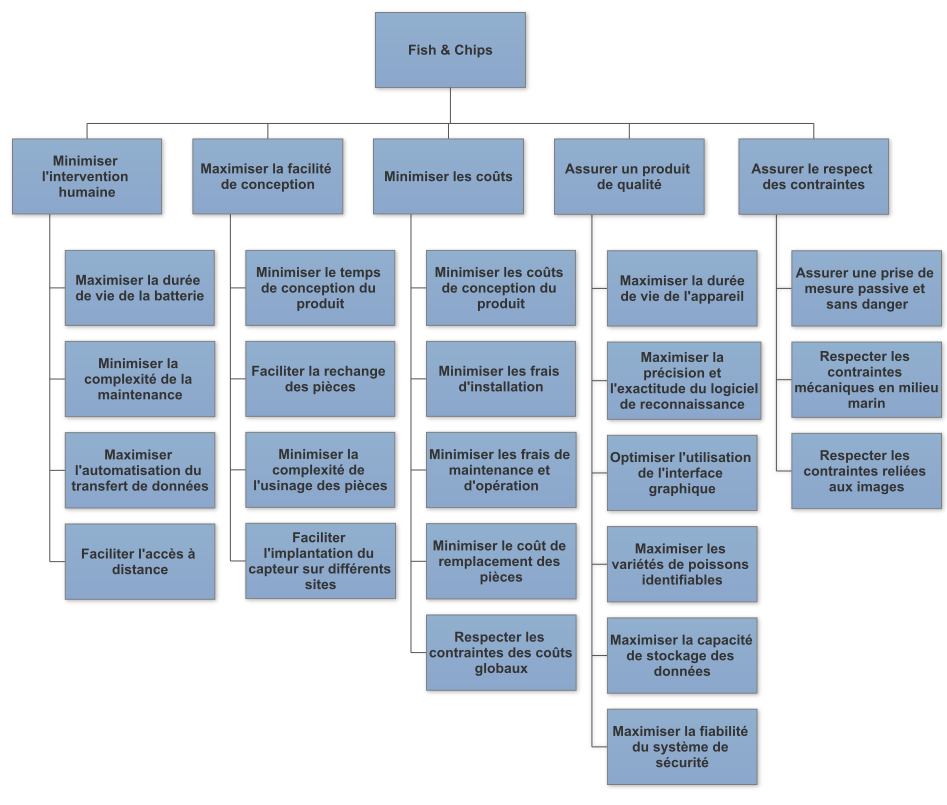
\includegraphics[width=1.0\linewidth]{fig/Organigramme.png}
        \caption{Organigramme des objectifs du projet Fish \& Chips}
        \label{fig:organigramme}
    \end{figure}
    
    %\item Autres (je sais pas dans quelle catégorie les mettre)
    %\begin{itemize}
    %    \item Maximiser la disponibilité du capteur
    %    \item Maximiser la sécurité
    %    \item Assurer une mesure passive
    %\end{itemize}
    
\end{enumerate}
